\documentclass[final,t,overlay, xcolor=table, sans, mathserif]{beamer}
\mode<presentation>
{
\usetheme{UCL}
}
\usepackage[orientation=landscape,size=a0,scale=1.15, debug]{beamerposter}
% \usepackage[orientation=landscape,size=custom, width=141, height=100,scale=1.2, debug]{beamerposter}
% \usepackage[orientation=landscape,size=custom,width=178,height=88.8,scale=1.6]{beamerposter}

% additional packages
\usepackage{tikz}
\usetikzlibrary{shapes,arrows}
\usepackage{paralist}
\setdefaultleftmargin{4.5em}{}{}{}{}{}
\usepackage{array}
\usepackage[english]{babel}
\usepackage[latin1]{inputenc}
\usepackage{wrapfig}
\usepackage{amsmath}
\usepackage{natbib}
\usepackage{multirow}
%\usepackage[pdftex]{graphicx}
\usepackage{epstopdf} 
\usepackage{xcolor}
\usepackage{tcolorbox}
%\usepackage{svg}
%\usepackage[inkscape={/Applications/Inkscape.app/Contents/Resources/bin/inkscap??e -z -C}]{svg}

%\usepackage{kerkis}
%\usepackage{kmath}


% additional settings
\setbeamerfont{itemize}{size=\normalsize}
\setbeamerfont{itemize/enumerate body}{size=\normalsize}
\setbeamerfont{itemize/enumerate subbody}{size=\normalsize}

\pdfpageattr{/Group << /S /Transparency /I true /CS /DeviceRGB>>}

% Define block styles
\tikzstyle{block} = [rectangle, draw, fill=blue!20,
    text width=8em, text centered, rounded corners, minimum height=4em]
\tikzstyle{arrow} = [thick,->,>=stealth]
%\tikzstyle{arrow} = [draw, very thick,color=black!50,-latex']

%\graphicspath{{fig/}}

% Display a grid to help align images
%\beamertemplategridbackground[1cm]



\title{Performance of synchrony and spectral-based features in early seizure detection:\\
exploring feature combinations and effect of latency.}
\author[Adam \& Soldado-Magraner]
{Vincent Adam$^1$, Joana Soldado Magraner$^1$, Wittawat Jitkrittum$^1$, Heiko Strathmann$^1$,
Balaji Lakshminarayanan$^1$, Alessandro Davide Ialongo$^1$, Gergo Bohner$^1$, Ben Dongsung Huh$^1$,\\
 Lea Goetz$^2$, Shaun Dowling$^3$, Iulian Vlad Serban$^3$, Matthieu Louis$^3$}
\institute[UCL]{The Gatsby Computational Neuroscience Unit$^1$, Wolfson Institute for Biomedical Research$^2$,
The Centre for Computational Statistics and Machine Learning$^3$ (CSML), UCL, London, UK.}

\date[IWSP7 2015]{IWSP7 2015}


\begin{document}
\begin{frame}{}


\begin{columns}[t]
%%%%%%%%%%%%% BEGIN COLUMN ONE %%%%%%%%%%%%%%%%%%%%%%%%%%%%%%%%%%%%%%%%%%%%
\begin{column}{.33\linewidth}



\begin{block}{Motivation}
\begin{itemize}
\item Accurate early \underline{\bf seizure detection} is crucial for building neurostimulation devices capable of
detecting the onset of seizures in order to stop their progress.
\item Availability of large scale intra-cranial EEG (iEEG) datasets and recent advances in {\bf machine learning}
 techniques make it possible to design efficient algorithms for this purpose.
\item The success of detecting seizures from recorded iEEG signals relies heavily on
 extracting discriminative \underline{\bf features} in the data which characterize different brain regimes.
\end{itemize}
\end{block}


\begin{block}{The data}
1 second multi-channel iEEG data segments from 8 human patients and 4 dogs with epilepsy was provided by the UPenn-Mayo Clinic
Seizure Detection Challenge, hosted on \emph{kaggle.com}, which was sponsored by the American Epilepsy Society. \\
\quad \\
The data was split into training and test sets.
\begin{itemize}
\item Training data segments were manually labelled as {\bf ictal} or {\bf interictal}.
\item Additionally, a segment was labeled {\bf early} if its time since seizure onset was below 15s.
\end{itemize}
\vspace{1cm}
\end{block}


\begin{block}{The task}
\centering
The task consisted on answering two questions about each test segment:
\begin{itemize}
\centering
\item[1.] Is it a seizure segment?
\item [2.] Is it an early seizure segment?
\end{itemize}
\end{block}



\begin{block}{The algorithm, in a nutshell}

\begin{center}
%\vspace{0.1cm}
It can be broken down in three main stages: \\
\vspace{1cm}
\begin{tikzpicture}[node distance = 2cm, auto]
    % Place nodes
    \node [block] (featext) {\bf{Feature \\ extraction}};
    \node [block, left of=featext, node distance=11cm] (prepro)  {\bf{Preprocessing}};
    \node [block, right of=featext, node distance=11cm] (class)  {\bf{Classification}};
    % Draw edges
    \draw [arrow, line width=0.3cm] (featext) -- (class);
    \draw [arrow, line width=0.3cm] (prepro) -- (featext);
\end{tikzpicture}
\end{center}

\centering
\begin{minipage}[t]{0.95\linewidth}
\begin{tcolorbox}[title=1. Preprocessing]
The signal was downsampled to 400Hz and low pass filtered with cutoff freq 400Hz. \\
Electrical noise in the band $59-61Hz$ was also removed.
\end{tcolorbox}
\end{minipage}

\begin{minipage}[t]{0.95\linewidth}
\begin{tcolorbox}[title=2. Feature extraction]
The aim is to obtain a set of parameters (feature vectors) which summarize the task-relevant statistics of the iEEG data.
\qquad \\

\begin{itemize}
\item {\bf Spectral energy (SE)} \\
Squared modulus of the signal's Fourier transform. Energy below $f_{max}=100Hz$ was averaged into $N_{bands}=40$ contiguous
bands of spectral width $\lfloor f_{max}/N_{bands}\rfloor$. \\
\qquad \\

\item {\bf Phase Locking Value (PLV)} \\
For each channel i, the instantaneous phase $\phi_{i}^{a}(t)$ of the analytical signal $x_{i}^{a}(t)$
of the time series $x_{i}(t)$ is extracted. Then, for each pair (i,j) of channels,
we compute: \\
$PLV_{ij}=\left|\frac{1}{T}\sum_{t}e^{i(\phi_{i}^{a}(t)-\phi_{j}^{a}(t))}\right|$ \\
\qquad \\

\item {\bf Vector autoregressive (VAR$\left[\tau\right]$) models} \\
The signal was modelled as: \\
$x_{t}=\sum_{k=1}^{\tau}A_{k}x_{t-k}+\epsilon_{t}, \epsilon\sim\mathcal{N}(0,Q)$ \\
The learned parameters $[A_{1},A_{2},...,A_{\tau},Q]$ were taken as features. \\
\qquad \\

\end{itemize}
\end{tcolorbox}
\end{minipage}


\begin{minipage}[t]{0.95\linewidth}
\begin{tcolorbox}[title=3. Clasification]
A Random Forest classifier was trained individually for each subject.
\end{tcolorbox}
\end{minipage}
\vspace{0.5cm}

\end{block}



\end{column}
%%%%%%%%%%%%% BEGIN COLUMN TWO %%%%%%%%%%%%%%%%%%%%%%%%%%%%%%%%%%%%%%%%%%%%
\begin{column}{.27\linewidth}


\begin{block}{Summary}
\quad \\
\vspace{0.2cm}
We extract a small set of features from the pre-processed iEEG signal based on {\bf neural synchrony} (VAR, PLV) and {\bf spectral energy} (SE).
We pair these features with a state-of-the-art random forest classifier to yield an algorithm
which is able to accurately identify ictal iEEG data segments and detect early periods of the seizures
({\bf latency} from seizure onset\textless15s). \\
\quad \\
\vspace{0.3cm}
\end{block}

\begin{block}{Analysis}
Once the classifier is trained:
\begin{itemize}
\item[I.] We evaluate the accuracy of the classifier in seizure detection and early seizure detection using the
Area Under the ROC Curve (AUC) as a metric. Furthermore, we analyse the {\bf importance of the different features}
for classification performance.
\item[II.] We compare the estimated probabilities of seizure and early seizure with respect to {\bf latency} to characterize
how accuracy changes as the seizure progresses.
\end{itemize}
\end{block}

\vspace{-0.2cm}
\begin{block}{Extracted features example.}
\begin{columns}
\column{0.49\textwidth}
\centering
{\bf \qquad \underline{ictal segment}}
\column{0.49\textwidth}
\centering
{\bf \quad \underline{inter-ictal segment}}
\end{columns}
\begin{figure}
\includegraphics[width=1\textwidth]{figures/features.pdf}
\end{figure}
\end{block}

\end{column}
%%%%%%%%%%%%% BEGIN COLUMN THREE %%%%%%%%%%%%%%%%%%%%%%%%%%%%%%%%%%%%%%%%%%%%
\begin{column}{.4\linewidth}

\begin{block}{Results I. Seizure \& early seizure detection performance}
\centering
\underline{\bf Overall performance, for all patients.}
\begin{columns}
\column{0.49\textwidth}
\vspace{-1cm}
\begin{figure}
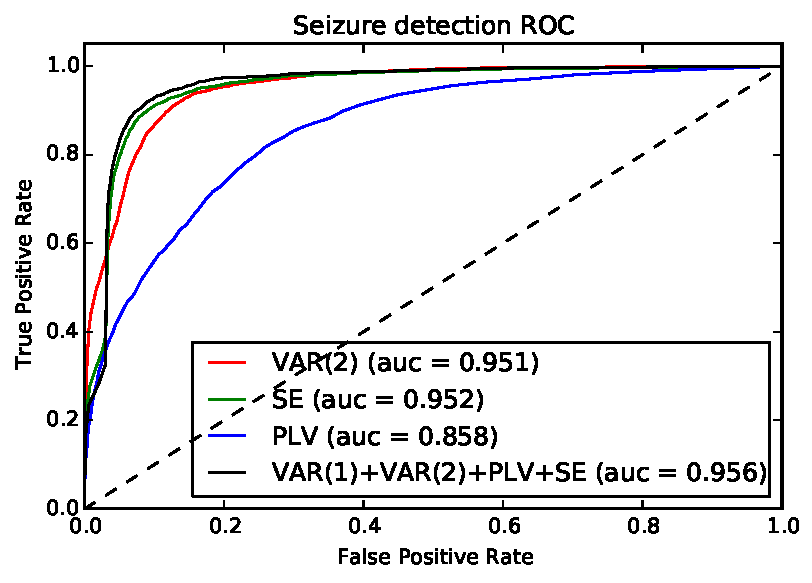
\includegraphics[width=1\textwidth]{figures/kaggle_2_train_test_ROCseizure.pdf}
\end{figure}
\column{0.49\textwidth}
\vspace{-1cm}
\begin{figure}
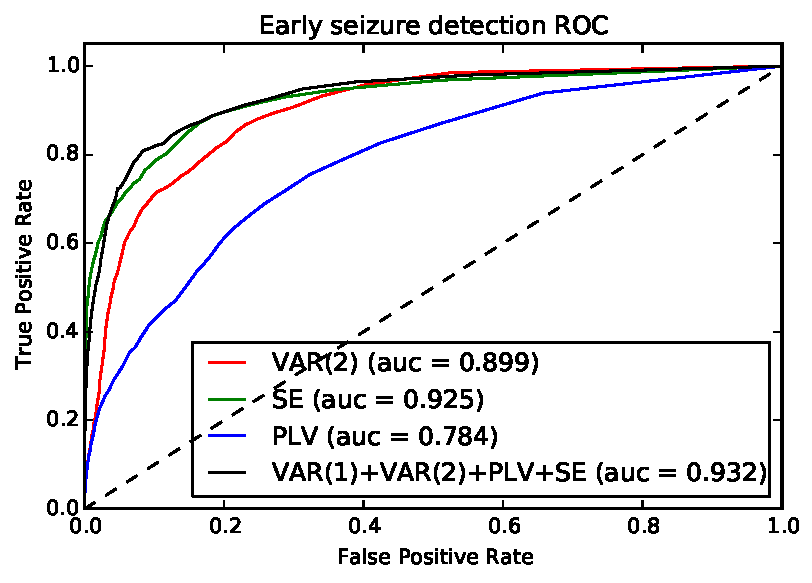
\includegraphics[width=1\textwidth]{figures/kaggle_2_train_test_ROCearly.pdf}
\end{figure}
\end{columns}

\centering
\underline{\bf Per-patient performance.} \\
\begin{columns}
\column{0.49\textwidth}
\vspace{-1cm}
\begin{figure}
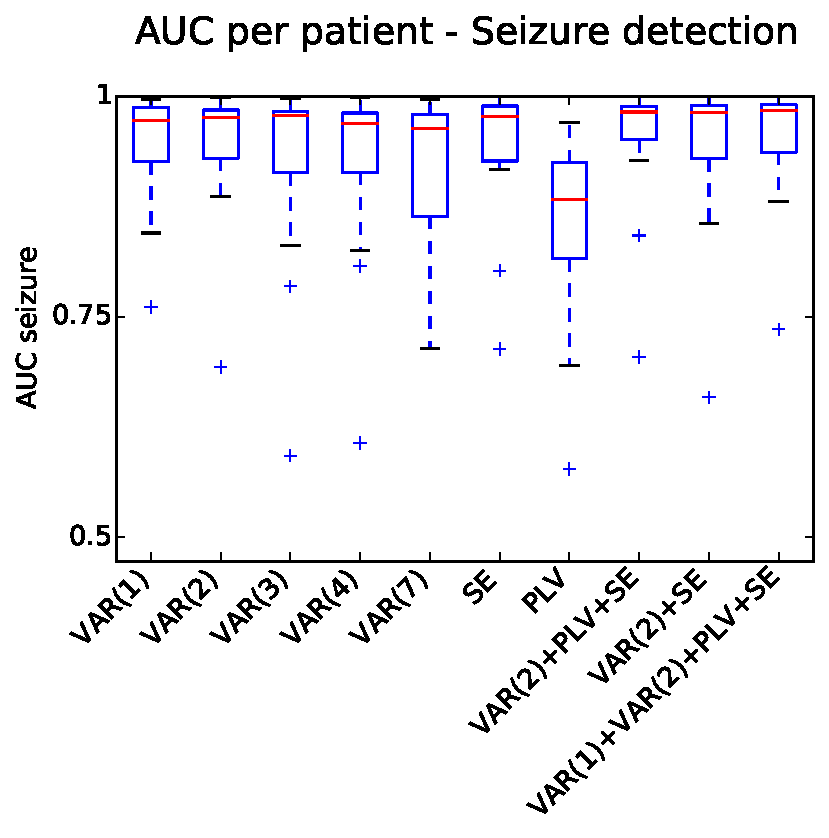
\includegraphics[width=0.9\textwidth]{figures/kaggle_2_train_test_seizure.pdf}
\end{figure}
\column{0.49\textwidth}
\vspace{-1cm}
\begin{figure}
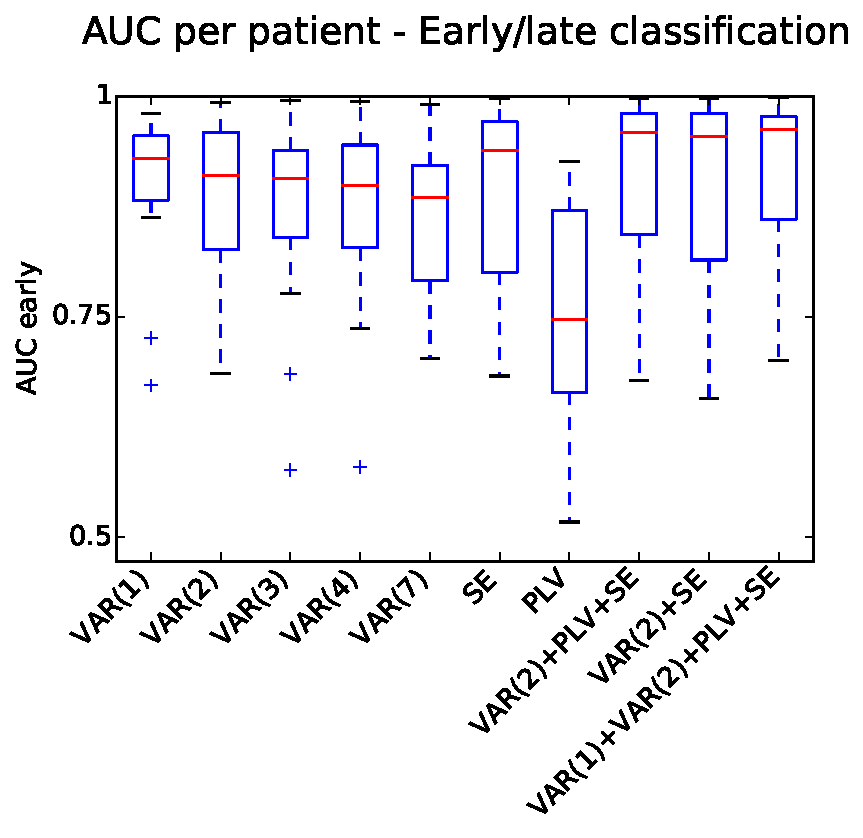
\includegraphics[width=0.9\textwidth]{figures/kaggle_2_train_test_early.pdf}
\end{figure}
\end{columns}
\end{block}

\vspace{-1.4cm}
\begin{columns}
\column{0.59\textwidth}
\begin{block}{Results II. Accuracy vs Latency.}
Patient example.
\begin{figure}
\includegraphics[width=0.5\textwidth]{figures/Patient_2_latency_seizure.pdf}
\includegraphics[width=0.5\textwidth]{figures/Patient_2_latency_early.pdf}
\end{figure}
\vspace{-0.8cm}
Dog example.
\begin{figure}
\includegraphics[width=0.5\textwidth]{figures/Dog_4_latency_seizure.pdf}
\includegraphics[width=0.5\textwidth]{figures/Dog_4_latency_early.pdf}
\end{figure}
\end{block}
\column{0.39\textwidth}
\begin{block}{Conclusions}
\begin{itemize}
\item Features extracted with VAR models beyond 2nd order do not improve classification performance.
\item A combination of SE+VAR+PLV achieves the best results in both tasks.
\item Data segments are more confidently classified as ictal as seizure progresses (latency).
\end{itemize}
\end{block}
\end{columns}



\end{column}
%%%%%%%%%%%%% END COLUMNS %%%%%%%%%%%%%%%%%%%%%%%%%%%%%%%%%%%%%%%%%%%%
\end{columns}


\end{frame}
\end{document}
